% Канонический TikZ-рисунок варианта 11. Править только здесь.
\long\def\figStereoV11{%
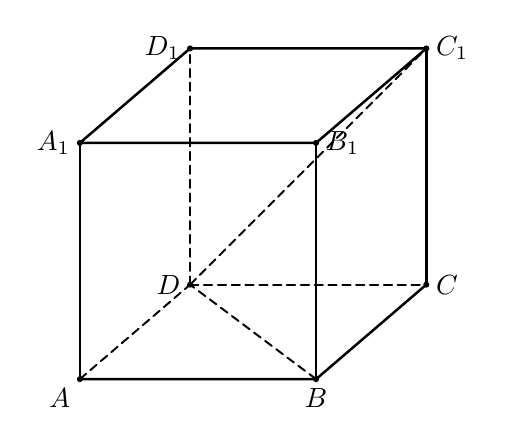
\begin{tikzpicture}[
    scale=1,
    line cap=round,
    line join=round,
    visible/.style={line width=0.9pt},
    hidden/.style={line width=0.7pt,dashed,dash pattern=on 3pt off 2pt}
]

% -------------------------------------------------
% Вершины куба
% Нижнее основание: ABCD
% Верхнее основание: A1B1C1D1
% -------------------------------------------------

\coordinate (A)  at (0,0);
\coordinate (B)  at (3,0);
\coordinate (C)  at (4.4,1.2);
\coordinate (D)  at (1.4,1.2);

\coordinate (A1) at (0,3);
\coordinate (B1) at (3,3);
\coordinate (C1) at (4.4,4.2);
\coordinate (D1) at (1.4,4.2);

% -------------------------------------------------
% Скрытые рёбра куба
% -------------------------------------------------

\draw[hidden] (A)--(D);
\draw[hidden] (D)--(C);
\draw[hidden] (D)--(D1);

% -------------------------------------------------
% Видимые рёбра куба
% -------------------------------------------------

\draw[visible] (A)--(B)--(C);
\draw[visible] (A)--(A1);
\draw[visible] (B)--(B1);
\draw[visible] (C)--(C1);

\draw[visible] (A1)--(B1)--(C1)--(D1)--cycle;
\draw[visible] (C1)--(C);

% -------------------------------------------------
% Нужные прямые
% -------------------------------------------------

% Диагональ основания BD
\draw[hidden] (B)--(D);

% Прямая DC1
\draw[hidden] (D)--(C1);

% -------------------------------------------------
% Подписи вершин
% -------------------------------------------------

\fill (A)  circle (1.1pt) node[below left]  {$A$};
\fill (B)  circle (1.1pt) node[below]       {$B$};
\fill (C)  circle (1.1pt) node[right]       {$C$};
\fill (D)  circle (1.1pt) node[left]        {$D$};

\fill (A1) circle (1.1pt) node[left]        {$A_1$};
\fill (B1) circle (1.1pt) node[right]       {$B_1$};
\fill (C1) circle (1.1pt) node[right]       {$C_1$};
\fill (D1) circle (1.1pt) node[left]        {$D_1$};

\end{tikzpicture}
}
